\setcounter{ExampleCounter}{1}
\subsection{Order of Operations}

When carrying out multiple operations (addition, multiplication, etc.) all at once, it is important to have a consistent order in which we do so.  For instance, consider the following string of operations:
\[7+3 \times 4 -6 \div\marginnote{This could also be written \[7+3 \cdot 4 - \dfrac{6}{2}\] by using $\cdot$ for multiplication and writing the division as a fraction.} 2\]
One person might want to add 7 and 3 first, then multiply that answer by 4, subtract 6 from that answer, and finally divide by 2.  In other words, they may want to simply go from left to right, carrying out operations as they go.

However, it turns out that we don't want to rely on the order in which things are written so much, so there is a consistent \textbf{order of operations} that, by convention, everyone doing mathematics should follow.

Take a look at a more complicated example:
\[(2-3)^2 - 8 \div 4 \cdot (2+1)\]

In general, there are six kinds of components here to worry about:
\begin{enumerate}
\item The \textbf{parentheses} form grouping statements.  As far as this book is concerned, that is all that parentheses do.
\item The \textbf{exponent} ($^2$) is simply a short-hand notation that means ``multiply this thing by itself.''  If the exponent looked like $^3$, it would mean ``multiply together three copies of this thing.''  In the example above, $(2-3)^2$ is the same as $(2-3)(2-3)$.  For more on exponents, look at Section R.4.
\item The \textbf{multiplication} can be written using either the $\times$ symbol or a simple dot: $\cdot$.  In fact, mathematicians are \textit{so} lazy that if we write two things with parentheses around them next to each other, like this:
\[(6)(12)\] we mean that they are being multiplied together.  We also do this with variables, so $6xy$, for instance, means 6 times $x$ times $y$.
\item The \textbf{division} can be written using either the $\div$ symbol or by writing a fraction.  For example, we could write \[9 \div 3 \textrm{ or } \dfrac{9}{3}.\]  In that example, we would call 9 the \textit{dividend} and 3 the \textit{divisor}, although we won't need that terminology much here.
\item The \textbf{addition} is always written with the plus sign.
\item Similarly, the \textbf{subtraction} is always written with the minus sign.
\end{enumerate}

Look back at that list.  The order in which the operations are listed there is the same as the order of operations.  Generally speaking, multiplication and division get taken care of before addition and subtraction, and parentheses and exponents come first.

To remember this, many people use an acronym formed from the first letters of each of these names: \textbf{PEMDAS}.
\begin{center}
{\huge\bfseries P}arentheses, {\huge\bfseries E}xponents, {\huge\bfseries M}ultiplication, {\huge\bfseries D}ivision, {\huge\bfseries A}ddition, {\huge\bfseries S}ubtraction
\end{center}

Therefore, to use this order of operations correctly, go from left to right through the expression, simplifying anything in parentheses.  Then, go through it again, handling all the exponents.  Then again, doing multiplication, and so on.
\pagebreak

\begin{example}{Order of Operations}
Evaluate the following expression:
\[7+3 \cdot 4 - \dfrac{6}{2}\]

\sol
There are no parentheses or exponents in this one, so we will start with the multiplication: replace $3 \cdot 4$ with 12.
\[7+12-\dfrac{6}{2}\]
Now, deal with the division: replace $\dfrac{6}{2}$ with 3.
\[7+12-3\]
Finally, add 12 to 7 and subtract 3 from the result:
\[19-3 = 16\]
Therefore,
\[7+3 \cdot 4-\dfrac{6}{2} = \boxed{16}\]
\end{example}

\begin{proc}{Using Your Calculator}
Most, if not all, calculators will use the correct order of operations if you enter an expression like this.
\begin{center}
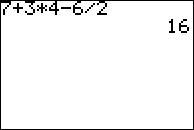
\includegraphics[height=1in]{Screen1}
\end{center}
However, it is never a bad idea to slow down and do one operation at a time, even using your calculator.  This can avoid errors that may arise if you try to enter a long expression into the calculator.
\end{proc}

\begin{example}{Order of Operations}
Evaluate the following expression:
\[(2-3)^2 - 8 \div 4 \cdot (2+1)\]

\sol
Remember \textbf{PEMDAS}\marginnote{\text{}\\ \text{}\\ Using the calculator:\\
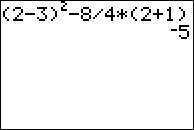
\includegraphics[scale=0.5]{Screen2}\\ Note: for the exponent, use the $\boxed{\wedge}$ key} first carry out any operations inside parentheses.
\[(2-3)^2 - 8 \div 4 \cdot (2+1) = (-1)^2 - 8 \div 4 \cdot 3\]
Next, apply the exponent: $(-1)^2$ is the same as $(-1) \cdot (-1)$ (which could also be written simply as $(-1)(-1)$).  This equals 1, because multiplying anything by $-1$ simply switches its sign.
\[1 - 8 \div 4 \cdot 3\]
Finally, apply the multiplication and division, and then the subtraction at the end:
\[1-8\div 4 \cdot 3 = 1 - 2 \cdot 3 = 1-6 = -5\]
Therefore, \[(2-3)^2 - 8 \div 4 \cdot (2+1) = \boxed{-5}\]
\end{example}

\begin{example}{Order of Operations}
Evaluate the following expression:
\[\dfrac{128-4(2+14)}{7+5^2}\]

\sol
This one looks a little bit different from the previous ones, but notice what's happening: the whole expression on the top is being divided by the whole expression on the bottom.  Really, then, these expressions are being \textit{grouped}, which means we could rewrite this using parentheses to show the grouping:
\[\dfrac{128-4(2+14)}{7+5^2} = (128-4(2+14)) \div (7+5^2)\]
Either way, we're going to first simplify the numerator and denominator separately, and divide them at the end.
\begin{align*}
\dfrac{128-4(2+14)}{7+5^2} &= \dfrac{128-4(16)}{7+5^2}\marginnote{\textbf{P}arentheses}\\
&= \dfrac{128-4(16)}{7+25}\marginnote{\textbf{E}xponents}\\
&= \dfrac{128-64}{7+25}\marginnote{\textbf{M}ultiplication}\\
&= \dfrac{64}{32}\marginnote{\textbf{A}ddition and \textbf{S}ubtraction}\\
&= \boxed{2}
\end{align*}
\end{example}

To do the preceding example with your calculator, use parentheses to group the numerator and denominator.
\begin{center}
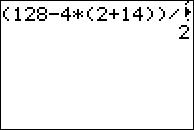
\includegraphics[scale=1]{Screen3}
\end{center}

\subsection{Distributing and Factoring}
Look at the following expression:
\[2(3+5).\]
Of course, using the proper order of operations, we could evaluate this by adding 3 and 5, before multiplying that answer by 2; this answer is 16.

However, what about an expression like the following one?
\[3(x-1)\]
Here, since $x$ is a variable, we can't subtract 1 from it.  But we \textit{can} simplify this by removing the parentheses: to do so, we need to \textbf{distribute} the 3 through the expression in the parentheses.  We do this by multiplying it by each term that appears in the parentheses:
\[3(x-1) = 3 \cdot x - 3 \cdot 1 = 3x-3\]

\begin{formula}{Distributing}
When multiplying one number by a sum or difference in parentheses, the multiplication can be \textbf{distributed} across the addition, as follows:
\[a(b+c) = ab + ac\]
or
\[a(b-c) = ab - ac\]
\end{formula}

\begin{example}{Distributing}
Distribute to remove the parentheses from the following expression.
\[4(5x-3)\]

\sol
Again, multiply the 4 by each term in the parentheses:
\[4(5x-3) = 4 \cdot 5x - 4 \cdot 3 = \boxed{20x-12}\]
\end{example}

\begin{example}{Distributing}
Distribute to remove the parentheses from the following expression.
\[-3(2x-9)\]

\sol
Here, the number that we distribute is negative.  This serves to flip the signs of each term inside the parentheses:
\[-3(2x-9) = (-3)(2x) - (-3)(9) = -6x - (-27)\marginnote{Notice that subtracting a negative number is the same as adding the opposite (positive) number} = \boxed{-6x+27}\]
\end{example}

The distribution rule can be reversed if that is useful in a particular problem: we can \textbf{factor} out a common factor from several terms.

\begin{formula}{Factoring}
If the terms in an expression are all multiples of the same number, that number can be \textbf{factored} out and written as a constant multiple of the remaining expression:
\[ab+ac = a(b+c)\]
\end{formula}

\begin{example}{Factoring}
Factor out any common factors from the following expression.
\[2x-6\]

\sol
Notice that both terms are multiples of 2 (2 divides into them evenly), so we can factor out the 2.  What will remain inside the parentheses is what remains when each term is divided by 2:
\[2x-6 = \boxed{2(x-3)}\]
\end{example}

Notice that sometimes we want to distribute to get rid of parentheses, and sometimes we want to factor, adding parentheses.  What we do depends on our goal: would we rather write an expression as a sum of several terms, with no grouping, or would we rather write it as a product, by factoring?  The answer, of course, depends on the kind of problem we're doing.  You should have both tools at your disposal, so that you can use either one when necessary.

\begin{example}{Factoring}
Factor out any common factors from the following expression.
\[3x^3+27x\]

\sol
This time, there is more than one thing common to both terms.  Notice that both are divisible by 3, and also that both contain a multiple of $x$.  Therefore, we can factor out the 3 \textit{and} the $x$:
\[3x^3+27x^2 = \boxed{3x(x^2+9)}\]
\end{example}

\subsection{Fractions}

We may need to add, subtract, multiply, or divide two fractions at some point.  First, we'll consider how to multiply and divide fractions, before seeing how to add and subtract them.

\begin{formula}{Multiplying Fractions}
To multiply two fractions, simply multiply their numerators to form the numerator of the answer, and multiply their denominators to form the denominator of the answer:
\[\dfrac{a}{b} \cdot \dfrac{c}{d} = \dfrac{ac}{bd}\]
\end{formula}

\begin{example}{Multiplying Fractions}
Carry out the following operation.
\[\left(\dfrac{1}{3}\right)\left(\dfrac{2}{5}\right)\]

\sol
Simply multiply straight across:
\[\left(\dfrac{1}{3}\right)\left(\dfrac{2}{5}\right) = \dfrac{(1)(2)}{(3)(5)} = \boxed{\dfrac{2}{15}}\]
\end{example}

\begin{example}{Multiplying Fractions}
Carry out the following operation.
\[\dfrac{15}{7} \cdot \dfrac{28}{3}\]

\sol
Again, multiply straight across.  This time, though, note that the final answer has common multiples in the numerator and denominator; these can be \textbf{canceled}.  To notice this, we will break 15 and 28 down into the smallest pieces multiplied together that we can:
\[\dfrac{15}{7} \cdot \dfrac{28}{3} = \dfrac{(15)(28)}{(7)(3)} = \dfrac{(3)(5)(2)(2)(7)}{(7)(3)} = \dfrac{\cancel{(3)}(5)(2)(2)\cancel{(7)}}{\cancel{(7)}\cancel{(3)}} = \dfrac{20}{1} = \boxed{20}\]
\end{example}
\vfill
\pagebreak

\begin{formula}{Dividing Fractions}
To divide two fractions, multiply the dividend by the \textbf{reciprocal} (flipped upside-down) of the divisor:
\[\dfrac{\dfrac{a}{b}}{\dfrac{c}{d}} = \dfrac{a}{b} \cdot \dfrac{d}{c}\]
Just remember: to divide two fractions, flip the bottom one upside down and multiply them.
\end{formula}

\begin{example}{Dividing Fractions}
Carry out the following operation.
\[\dfrac{2}{3} \div \dfrac{4}{3}\]

\sol
Flip the divisor and change the division to multiplication:
\[\dfrac{2}{3} \div \dfrac{4}{3} = \dfrac{2}{3} \cdot \dfrac{3}{4} = \dfrac{(2)(3)}{(3)(4)} = \dfrac{(2)\cancel{(3)}}{\cancel{(3)}(4)} = \dfrac{2}{4} = \boxed{\dfrac{1}{2}}\]
\end{example}

\begin{example}{Dividing Fractions}
Carry out the following operation.
\[\dfrac{5}{\dfrac{1}{6}}\]

\sol
Even though this one doesn't look like we're dividing two fractions, the numerator can also be written as 5/1, which is a fraction:
\[\dfrac{\dfrac{5}{1}}{\dfrac{1}{6}} = \dfrac{5}{1} \cdot \dfrac{6}{1} = \dfrac{30}{1} = \boxed{30}\]
\end{example}

\begin{formula}{Adding and Subtracting Fractions}
To add or subtract two fractions, the two fractions must have a common denominator.  If so, simply add/subtract the numerators and keep the common denominator:
\[\dfrac{a}{c} + \dfrac{b}{c} = \dfrac{a+b}{c}\]
\[\dfrac{a}{c} - \dfrac{b}{c} = \dfrac{a-b}{c}\]

If the two fractions do not have a common denominator, multiply each fraction by something of the form $\dfrac{d}{d}$ as needed to give them a common denominator.
\end{formula}
\pagebreak

\begin{example}{Adding and Subtracting Fractions}
Carry out the following operation.
\[\dfrac{1}{3} - \dfrac{5}{3}\]

\sol
Since these have the same denominator, we can simply subtract the numerators ($1-5 = -4$), and write\marginnote{Notice that $\frac{-4}{3} = - \frac{4}{3}$, since a negative number divided by a positive number gives a negative answer.} that over the common denominator:
\[\dfrac{1}{3} - \dfrac{5}{3} = \boxed{-\dfrac{4}{3}}\]
\end{example}

\begin{example}{Adding and Subtracting Fractions}
Carry out the following operation.
\[\dfrac{3}{4} + \dfrac{2}{3}\]

\sol
This time, the fractions do not have a common denominator, so we must rewrite them so that they do.  We can do this by multiplying the top and bottom of a fraction by the same amount.\marginnote{Note: sometimes, rather than multiplying by each other, we can pick smaller multiples to achieve our goal.  This is called finding the \textbf{least common denominator (LCD)}.  For instance, if it were 3/4 + 1/8, we could multiply the first by 2/2 and leave the second unchanged; both would have a denominator of 8.}\\

Thus, we want to multiply 4 by something and 3 by something else so that the two answers are identical.  If we multiply them by each other, this will be guaranteed to work.

\[\dfrac{3}{4} \cdot \dfrac{3}{3} + \dfrac{2}{3} \cdot \dfrac{4}{4} = \dfrac{9}{12} + \dfrac{8}{12} = \dfrac{9+8}{12} = \boxed{\dfrac{17}{12}}\]
\end{example}

\begin{exercises}
\textit{In exercises 1--8, use the correct order of operations to simplify each expression.  Do not rewrite any fractions as decimals.  You may use your calculator to check your work after doing it by hand.}

\pfour{$(5)(6)-10 \div 2+1$}
\pfour{$5+44-(6+8\div 2) + (2)(3)$}
\pfour{$-3^2 + 2 \cdot 3 + 10$}
\pfour{$5-(2+3)^2+(8)(2) \div 4$}

\pfour{$\dfrac{5-4}{7-(-2)}$}
\pfour{$\dfrac{5-(-3)}{-2-(-7)}$}
\pfour{$\dfrac{(-5)(3)+4^2}{6+3^2}$}
\pfour{$\dfrac{15 \div 5 \cdot 4 \div 6 - 8}{-6 - (-5) - 8 \div 2}$}

\textit{In exercises 9--16, distribute to remove the parentheses from each expression.}

\pfour{$2(x+1)$}
\pfour{$4(5-2y)$}
\pfour{$-7(2w-3)$}
\pfour{$(x+4)(-3)$}

\pfour{$\dfrac{1}{2}x(2y-8)$}
\pfour{$3.1(2p+1.5)$}
\pfour{$5(2x+y-3)$}
\pfour{$3x(5xy+7y-13)$}

\textit{In exercises 17--24, factor out any common factors from each expression.}

\pfour{$x^2+4x$}
\pfour{$3a-15$}
\pfour{$4+12y$}
\pfour{$8x-14$}

\pfour{$2+4x+8x^2$}
\pfour{$16-18y^3$}
\pfour{$5y-25y^2$}
\pfour{$6x^2y-15xy^2$}

\textit{In exercises 25--36, carry out the given operation and write each fraction in lowest terms, but do not write fractions as decimals.}

\pfour{$\left(\dfrac{1}{9}\right)\left(\dfrac{3}{4}\right)$}
\pfour{$\left(\dfrac{2}{3}\right)\left(\dfrac{1}{5}\right)$}
\pfour{$\dfrac{5}{6} \cdot \dfrac{3}{2}$}
\pfour{$\dfrac{1}{3}\left(\dfrac{6}{5} - \dfrac{3}{10}\right)$}

\pfour{$\dfrac{\dfrac{7}{5}}{\dfrac{3}{5}}$}
\pfour{$\dfrac{\dfrac{4}{9}}{5}$}
\pfour{$\dfrac{4}{5} \div \dfrac{2}{3}$}
\pfour{$\dfrac{\dfrac{2}{5} + \dfrac{3}{10}}{2}$}

\pfour{$\dfrac{3}{8} + \dfrac{7}{8}$}
\pfour{$\dfrac{6}{35} - \dfrac{3}{20}$}
\pfour{$\dfrac{2}{15} + \dfrac{6}{25}$}
\pfour{$\dfrac{9}{24} - \dfrac{3}{5}$}

\vspace*{0.25in}

{\color{blue!60!black} \rule{\textwidth}{3pt}}
\vspace*{0.25in}
\vfill
\pagebreak

\subsection{Answers}
\renewcommand*{\thefootnote}{\fnsymbol{footnote}}
\begin{tabularx}{\textwidth}{l l l l l l}
1. $26$ & 2. {$45$} & 3.\footnote{(note the lack of parentheses around $-3$)} $7$ & 4. {$-16$} & 5. {$\dfrac{1}{9}$} & 6. {$\dfrac{8}{5}$}\\ \\
7. {$\dfrac{1}{15}$} & 8. {$\dfrac{6}{5}$} & 9. {$2x+2$} & 10. {$20-8y$} & 11. {$-14w+21$} & 12. {$-3x-12$}\\ \\
13. {$y-4$} & 14. {$6.2p+4.65$} & 15. {$10x+5y-15$} & 16. {$15x^2y+21xy-39x$} & 17. {$x(x+4)$} & 18. {$3(a-5)$}\\ \\
19. {$4(1+3y)$} & 20. {$2(4x-7)$} & 21. {$2(1+2x+4x^2)$} & 22. {$2(8-9y^3)$} & 23. {$5y(1-5y)$} & 24. {$3xy(2x-5y)$}\\ \\
25. {$\dfrac{1}{12}$} & 26. {$\dfrac{2}{15}$} & 27. {$\dfrac{5}{4}$} & 28. {$\dfrac{3}{10}$} & 29. {$\dfrac{7}{3}$} & 30. {$\dfrac{4}{45}$}\\ \\
31. {$\dfrac{6}{5}$} & 31. {$\dfrac{7}{20}$} & 33. {$\dfrac{5}{4}$} & 34. {$\dfrac{3}{140}$} & 35. {$\dfrac{28}{75}$} & 36. {$-\dfrac{27}{120}$}
\end{tabularx}
\renewcommand*{\thefootnote}{\arabic{footnote}}
\setcounter{footnote}{0}
\end{exercises}